\documentclass[11pt]{article}
\renewcommand{\baselinestretch}{1.05}
\usepackage{amsmath,amsthm,verbatim,amssymb,amsfonts,amscd, graphicx}
\usepackage{graphics}
\topmargin0.0cm
\headheight0.0cm
\headsep0.0cm
\oddsidemargin0.0cm
\textheight23.0cm
\textwidth16.5cm
\footskip1.0cm
\theoremstyle{plain}
\newtheorem{theorem}{Theorem}
\newtheorem{corollary}{Corollary}
\newtheorem{lemma}{Lemma}
\newtheorem{proposition}{Proposition}
\newtheorem*{surfacecor}{Corollary 1}
\newtheorem{conjecture}{Conjecture} 
\newtheorem{question}{Question} 
\theoremstyle{definition}
\newtheorem{definition}{Definition}
\usepackage[document]{ragged2e}
\DeclareMathOperator{\Ima}{Im}
\begin{document}
 
\title{Lab 3}
\author{Zeyuan Xu}
\maketitle

\section{Task 1}
denote $x$ as the $(d+1)$ vector and $W$ as the $r \times (d+1)$ matrix, with each row $w_i \in \mathbb{R}^{d+1}, i\in \{ 1,..., r\}$ Then the decision boundary between class i and class j is given by the case where  $f(x)$ gives the same result for input $x$ at column $i$ and $j$, which is equivalently when $w_i^\top x = w_j^\top x$: \begin{align*}
f_i(x, w_i) = f_j(x, w_j) \Longrightarrow (w_i - w_j)^
\top x = 0
\end{align*}

\section{Task 2}
It does make sense to use a linear classifier, since from the plot, it looks like a line could separate the blue and red points. The plot is shown in figure 1. 

\section{Task 3}
The least square coefficient is computed by the formula \begin{align*}
W = (X^\top X)^{-1} X^\top T = \begin{bmatrix}
-0.2217 & -0.3236 & 1.8168 \\
0.2217 & 0.3236 & -0.8168
\end{bmatrix}
\end{align*}
where $T$ is a 100 by 2 matrix, where the first 50 rows are $[1,0]$, and 50-100 rows are $[0,1]$. The resulting matrix is 2 by 3 matrix. 
The decision boundary plot is shown in figure 2. 
\begin{figure}[!htb]
   \begin{minipage}{0.48\textwidth}
     \centering
     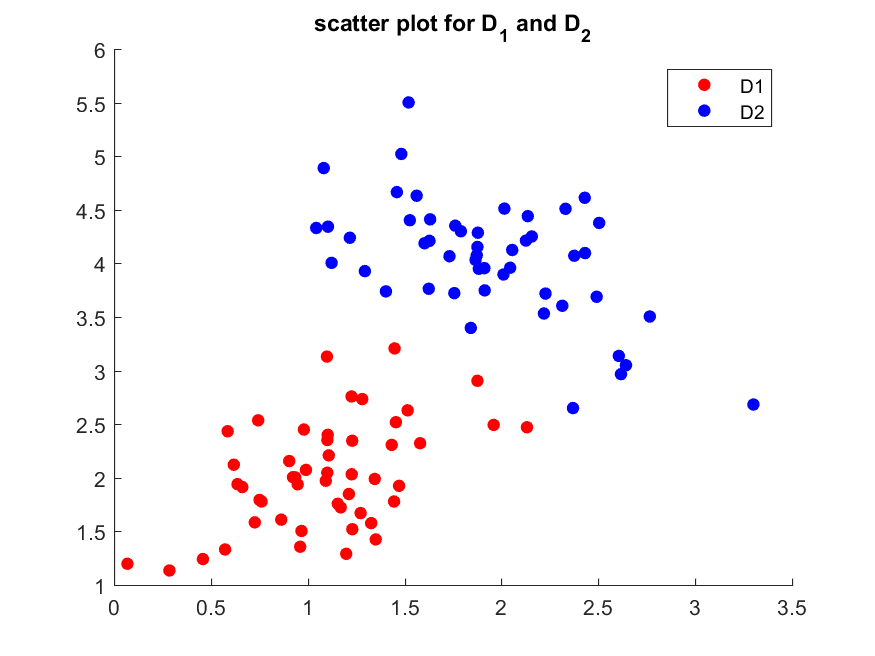
\includegraphics[width=.7\linewidth]{Task2.png}
     \caption{Scatter plot}\label{Fig:Original image}
   \end{minipage}\hfill
   \begin {minipage}{0.48\textwidth}
     \centering
     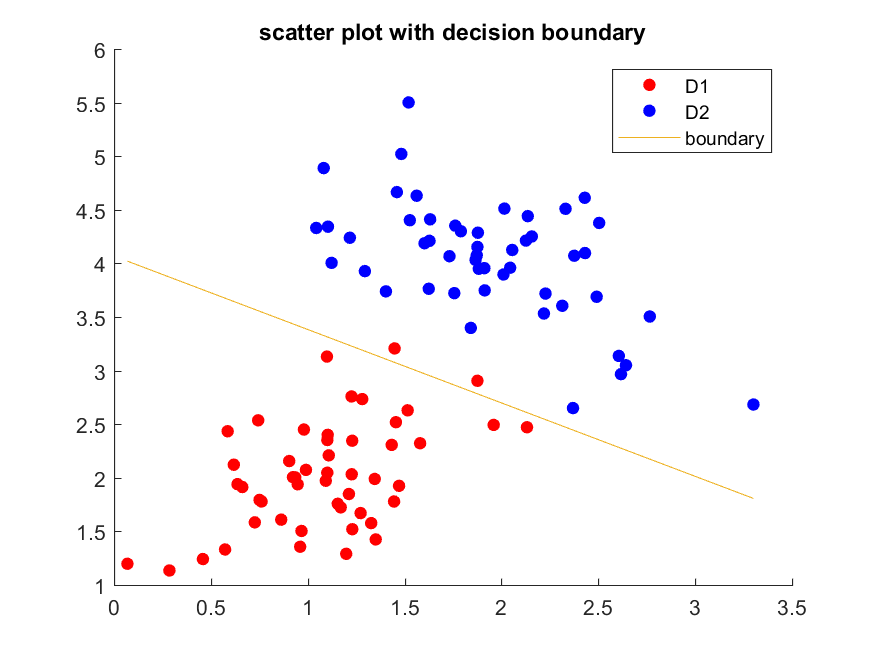
\includegraphics[width=.7\linewidth]{Task3.png}
     \caption{Scatter plot with boundary}\label{Fig:Rotate 90 degrees}
   \end{minipage}\hfill 
\end{figure} 

\section{Task 4}
The classification accuracy for $W$ in my case is $100$ percent. This result is tested given the newly generated datasets, which should also have first 50 rows as one class and 50-100 as the other class. This is quite surprising since from the previous generated datasets, two red points are on the blue side of the boundary. 

\section{Task 5}
The computed $W$ in this case is a 3 by 3 matrix: \begin{align*}
W =\begin{bmatrix}
-0.3142 & -0.0987 & 0.4129 \\
-0.4015 & 0.3369 & 0.0647 \\
2.2754 & -0.4508 & -0.8246
\end{bmatrix}
\end{align*}
The plot is shown in figure 3. The decision boundary is hand-drawn.
\begin{figure}
  \centering 
  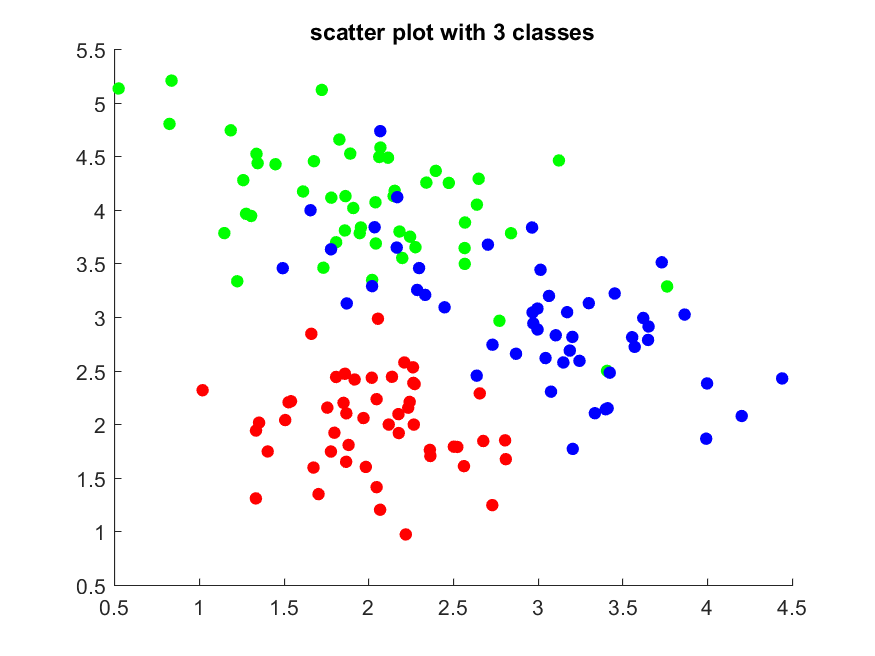
\includegraphics[width= \linewidth]{Task5.png}
  \caption{3 class scatter plot}
  \label{fig:3 classes}
\end{figure}

\section{Task 6}
in the 150 data samples, 87 are misclassified. This is a success rate of 42 percent. It is rather low, but jugding from figure 3, it is reasonable, because alot of points are mixed between green dots and blue dots. 

\section{Task 7}
The result of K Nearest Neighbor (with Matlab's built-in \textbf{knnsearch} function) is as follows: As k grows from 1 to 15, The number of incorrect classifications are: 30, 24, 23, 18, 19, 20, 18, 17, 19, 17, 17, 17, 21, 19, 19. This translates to accuracy of: \%80, \%84, \%84.67, \%88, \%87.33, \%86.67, \%88, \%88.67, \%87.33, \%88.67, \%88.67, \%88.67, \%86, \%87.33,\%87.33. Therefore, the overall accuracy is much better than the linear classifier in Task 6, which has only 42 percent accuracy. The K nearest neighbor method performs better in this case, because KNN is essentially a non-linear classification method, and in this case, given that the 3 datasets have some overlaps, it is better to use nonlinear boundary rather than linear ones. Also, since we have 3 classes, and a line can only cut the space in 2 parts, but in this case, we need to partition the space into 3 sets, linear model thus does not work very well. 

\end{document}